\documentclass[11pt,a4paper,twocolumn]{article}
\usepackage[utf8]{inputenc}
\usepackage{amsmath}
\usepackage{amsfonts}
\usepackage{amssymb}
\usepackage{hyperref}
\usepackage{graphicx}
\usepackage{caption}
\usepackage{subcaption}
\usepackage[left=1in,right=1in,top=1in,bottom=1in]{geometry}
\author{Daniel Deutsch and Dan Crankshaw}
\title{Machine Learning: Final Paper}
\date{}
\begin{document}
\maketitle

\section{Introduction}

A common problem in the field of machine learning is correctly identifying
handwritten words. The applications of
such a model are clear, and have already been implemented in situations like
the US postal service to sort mail based on the zip code.

The idea behind our approach is to compare how well two algorithms perform in
completing the optical character recognition task. The first algorithm is an
artifical neural network that will try to classify characters based on
their pixel values. The second algorithm is a combination of the previous
neural network and a hidden markov model, which will take into account the
probability of specific letter combinations. We hope that the addition of contextual
about the surrounding letters will help improve the accuracy of the neural
network.

\section{Related Work}

\emph{Other Paper} \cite{feng2008hidden}

\section{The Algorithms and Data}

\subsection*{Data}

The data that will be used in the training and evaluation of the ANN and the HMM was gathered from
\href{http://ai.stanford.edu/~btaskar/ocr/}{an optical character recognition dataset from
Stanford University}.
The data is a collection of handwritten letters segemented from words in which all uppercase
characters have been removed. We took the raw data and removed specific features included in the
data that we intended not to use. The resulting data set is a list of binary pixel values of each
character's 16 by 8 image.  \begin{figure}[h]
    \centering
    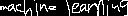
\includegraphics{img/ml.jpg}
    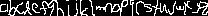
\includegraphics{img/alphabet.jpg}
    \caption{An example of the data set}
\end{figure}

The data can often be difficult to read for a human as Figure 1 demonstrates.
Although it is possible to make out each letter, this task is made much
easier by looking at the context of the word and anticipating what the letter
should be. The figure also illustrates that many of the same letters are a
variety of different sizes and are placed at different locations within the
image. The quality of the data may make it difficult for the ANN to learn how
to recognize each letter. However, the combination of the ANN and the HMM may
be a good simulation of how a human would approach the problem: try to
recognize the letter, then use context clues to figure out which character it
is.

The corpus used to learn the transmission probabilities for the HMM is a
a Project Gutenberg plain-text copy of \emph{Moby Dick}. We cleaned the
corpus by converting all letters to lowercase and removing all non-alphabetic
characters (i.e.\ numbers and punctuation). Our training corpus is the first
half of the text and the test corpus is the second half of the text.

\subsection*{The Algorithms}

The two algorithms that we intend to use to accomplish the word
recognition goal are an artificial neural network (ANN) and a hidden Markov
model (HMM). The idea is to compare the accuracy of the ANN to a combination of
both the ANN and HMM to see if adding knowledge of letter context to the model
increases accuracy on the datasets.

The ANN will be trained on the pixel values for each letter image. Each
training example is a 16 by 8 pixel image which amounts to an input size of
128. In order to help improve the accuracy of the classifier, we included a
bias term on the input and hidden layers. Therefore, the input size for the ANN
is 129 nodes.

Similarly, since we are trying to classify each image as a letter, there will
need to be 26 output nodes, one for each lowercase letter in the alphabet.
Therefore, the input and output sizes are set. The only parameters left to tune
for the ANN are the number of hidden layers and the number of nodes within each
hidden layer.

In order to find the best values for these parameters, we ran a series of tests
on the development data set to try and tune the parameters. We compared the
accuracies of each model on the development dataset to try and find the optimal
parameters.

The following was generated by randomly initializing an ANN with the given
hidden layer sizes, then training them all on the same data. This process is
repeated 20 times per data point, and the average accuracy is given. The
accuracy is determined by if the classifier gets the data point exactly
correct. Another common metric is to test if it got the right answer within the
top 5 guesses, but that is not used here.

For the ANN with one hidden layer, the only parameter than can be changed is the number of
hidden nodes in that layer.
\begin{figure}[h]
    \caption{Accuracies of two-layer networks}
    \centering
    \begin{tabular}{|c|c|}
        \hline 
        Hidden Nodes & Accuracy \\ 
        \hline 
        25 & 54.86\% \\ 
        \hline 
        50 & 54.24\% \\ 
        \hline 
        75 & 52.13\% \\ 
        \hline 
    \end{tabular} 
\end{figure}

Since all three data points are relatively similar, and the smaller neural
network will train faster, we will use a network with one hidden layer and 25 nodes
in that layer.

This data is indicative of our belief that the neural network might have some
difficultly classifying this dataset. The input seems to be a relatively
difficult dataset with some noise. Since adding more nodes to the hidden layer
did not imporve the accuracy significantly enough, it's evident that the
network is having a hard time learning the data. It may have reached its
maximal ability to learn. We hope that the combination of the HMM with the ANN
will help improve these accuracies.

One other idea that we tried was to add a second hidden layer to see if
increasing the number of weights allowed for improvement. With a small number
of tests, the amount of improvement was almost non-existent. Therefore, given
the extra amount of time it takes to train a neural network with two hidden
layers, we concluded that it was not worth the investment.

Therefore, the neural network that we will use in our experiments in
combination with and against the HMM will be a neural network with 128 input
nodes, 25 hidden nodes, and 26 output nodes, not counting the bias units.

We trained the HMM in a supervised setting, directly learning the parameters
from labeled data. We treat the actual letters that make up a word as the
hidden nodes ($z_i$) and the letters predicted by the ANN based on that
input as the observed nodes ($x_i$). The first set of parameters that the HMM
needs to learn are the emission probabilities $P(x_i | z_j)$. This is the probability
that the ANN predicts an observed letter $x_i$ given a letter representing
the state $z_j$. We learn these probabilities 

ADD DISCUSSION OF THEORY BEHIND HMM
ADD NOTE ABOUT LEARNING EMISSION PROBS BAYESIAN VS NON BAYESIAN


\section{Results}

\section{Analysis}

\section{Conclusion}

\bibliography{refs.bib}
\bibliographystyle{plain}

\end{document}
